\documentclass{VUMIFPSmagistrinis}
% \usepackage{algorithmicx}
% \usepackage{algorithm}
% \usepackage{algpseudocode}
\usepackage{amsfonts}
\usepackage{amsmath}
\usepackage{bm}
\usepackage{caption}
\usepackage{color}
\usepackage{float}
\usepackage{graphicx}
\usepackage{listings}
\usepackage{subfig}
\usepackage{wrapfig}

% Default settings for code listings
\lstset{frame=tb,
  language=scala,
  captionpos=b,
  aboveskip=3mm,
  belowskip=3mm,
  showstringspaces=false,
  columns=flexible,
  basicstyle={\small\ttfamily},
  numbers=none,
  numberstyle=\tiny\color{gray},
  %keywordstyle=\color{blue},
  %commentstyle=\color{dkgreen},
  %stringstyle=\color{mauve},
  frame=single,
  breaklines=true,
  breakatwhitespace=true
  tabsize=3
}

\renewcommand{\lstlistingname}{Kodo pavyzdys}

% Titulinio aprašas
\university{Vilniaus universitetas}
\faculty{Matematikos ir informatikos fakultetas}
\department{Programų sistemų katedra}
\papertype{Magistro baigiamasis darbas}
\title{Reaktyvus programavimas įvykių kaupimo sistemose}
\titleineng{Reactive Programming in Eventsourcing Systems}
\author{Žilvinas Kučinskas}
% \secondauthor{Vardonis Pavardonis}   % Pridėti antrą autorių
\supervisor{Viačeslav Pozdniakov}
\reviewer{prof. Rimantas Vaicekauskas}
\date{Vilnius – \the\year}

% Nustatymai
% \setmainfont{Palemonas}   % Pakeisti teksto šriftą į Palemonas (turi būti įdiegtas sistemoje)
\bibliography{bibliografija}

\begin{document}
\maketitle

%% Padėkų skyrius
% \sectionnonumnocontent{}
% \vspace{7cm}
% \begin{center}
%     Padėkos asmenims ir/ar organizacijoms
% \end{center}

\sectionnonumnocontent{Santrauka}
Glaustai aprašomas darbo turinys: pristatoma nagrinėta problema ir padarytos
išvados. Santraukos apimtis ne didesnė nei 0,5 puslapio. Santraukų gale
nurodomi darbo raktiniai žodžiai.
Nurodomi iki 5 svarbiausių temos raktinių žodžių (terminų).
Vienas terminas gali susidėti iš kelių žodžių.
\raktiniaizodziai{raktinis žodis 1, raktinis žodis 2, raktinis žodis 3, raktinis žodis 4, raktinis žodis 5}

\sectionnonumnocontent{Summary}
Santrauka anglų kalba. Santraukos apimtis ne didesnė nei 0,5 puslapio.
\keywords{keyword 1, keyword 2, keyword 3, keyword 4, keyword 5}

\tableofcontents

\sectionnonum{Įvadas}
Įvade aprašomi darbo tikslai, nurodomas temos aktualumas, aptariamos teorinės
darbo prielaidos bei metodika, apibrėžiamas tiriamasis objektas,
apibūdinami su tema susiję literatūros ar kitokie šaltiniai, temos analizės
tvarka, darbo atlikimo aplinkybės, pateikiama žinių apie naudojamus
instrumentus (programas ir kt.). Darbo įvadas neturi būti dėstymo santrauka.
Įvado apimtis 3-4 puslapiai.

\section{Magistro darbo objekto apžvalga bei tyrimo problemos aprašymas}
\subsection{Tyrimo objektas}

    Tyrimo objektas yra reaktyvaus programavimo bei įvykių kaupimo principai. Reaktyvus programavimas yra susijęs su reaktyviomis sistemomis, o kalbant apie įvykių kaupimo sistemas, įvykių kaupimo principas yra dažniausiai neatsiejamas nuo komandų-užklausų atsakomybių atskyrimo principo. Dėl to reikia apžvelgti ir pačią sistemą, įkomponuojančią šiuos principus, jog būtų galima susidaryti sistemos architektūros (aukštesnės abstrakcijos) vaizdą, analizuoti panaudojimo atvejus bei aprašyti tokių sistemų kūrimo gaires.

\subsection{Darbo tikslas}

  Darbo tikslas yra pritaikyti reaktyvaus programavimo principus įvykių kaupimo sistemose taip, jog skaitymo modelis būtų kuriamas tik komponavimo būdu, neturėtų būsenos, tai yra visos operacijos su duomenų baze būtų paslėptos, o programinis kodas - griežtai tipizuotas.

  % Darbo tikslas yra pritaikyti reaktyvaus programavimo principus įvykių kaupimo sistemose taip, jog būtų išpildyti šie reikalavimai:

  % \begin{itemize}

  %   \item reaktyviojo programavimo programos sąsaja (API) būtų valdoma atgalinių iškvietimų.

  %   \item reaktyviojo programavimo programos sąsaja (API) būtų deklaratyvi, tai yra leistų naudoti reaktyvius operatorius.

  %   \item įvykių kaupimo sistemos skaitymo modelis būtų kuriamas naudojant reaktyviojo programavimo programos sąsają (API).

  %   \item įvykių kaupimo sistemos skaitymo modelį būtų galima kurti asinchroniškai.

  %   \item naudojant reaktyviojo programavimo programos sąsają (API) būtų galima kurti Reaktyvumo manifeste aprašytas reaktyvias sistemas, tai yra būtini bruožai būtų išpildomi (atkuriamumas, reagavimas į įvykius, našumas).

% \end{itemize}

\subsection{Darbo uždaviniai}

  Siekiant tikslo, turi būti išspręsti šie uždaviniai:

\begin{itemize}
  \item išnagrinėti egzistuojančią (-ias) reaktyvaus programavimo biblioteką (-as).
  \item išnagrinėti egzistuojančią (-ias) įvykių kaupimo biblioteką (-as) ar programavimo karkasą (-us).
  \item sukurti konceptualų architektūros modelį, apjungiantį reaktyvų programavimą bei įvykių kaupimo principus, aprašyti praktines įvykių kaupimo sistemos kūrimo gaires.
  \item sukurti arba praplėsti esamą konkretizuotą kalbą (angl. domain specific language), apjungiančią reaktyvaus programavimo bei įvykių kaupimo principus.
  \item aprašyti konkretizuotuos kalbos kūrimo metodiką, apibrėžti gautų rezultatų apribojimus, suformuluoti iškilusias problemas bei paaiškinti jų priežastis.
  \item sukurti pavyzdinę programą bei įvertinti alternatyvius būdus kurti skaitymo modelį.
\end{itemize}

\subsection{Darbo nauda įgyvendinus tikslą}

\textbf{Akademinė}:

\begin{itemize}
  \item sukurtas inovatyvus arba alternatyvus būdas kurti skaitymo modelį įvykių kaupimo sistemose deklaratyviai, paslėpiant veiksmus su duomenų saugykla.
  \item medžiagą būtų galima naudoti dėstant apie įvykių sistemas, turėti  tokių reaktyvių sistemų kūrimo gaires, pritaikomas praktinių užsiėmimų metu.
\end{itemize}

\textbf{Verslo}:

\begin{itemize}
  \item Sukurtas pavyzdinis projektas, paruoštas naudoti produkcijos gamybos aplinkoje - sutaupytų daug laiko, nes nereikėtų konfigūruoti aplinkos nuo nulio.
\end{itemize}

Kadangi reaktyvus programavimas leidžia kurti sistemas komponavimo būdu, deklaratyviai, pasiekus tikslą būtų galima supaprastinti įvykių kaupimu pagrįstų sistemų kūrimą, struktūrizuoti kodą į smulkesnius, lengviau suprantamus ir palaikomus komponentus.

% Toks atskyrimas leistų atlikti panašią paskirtį kaip modelio-kontrolieriaus-vaizdo projektavimo šablono maršrutizatorius. Būtų galima apsirašyti kas ir kokius įvykius apdoroja su papildoma galimybe filtruoti ir transformuoti gautus įvykius.

\subsection{Tyrimo aktualumas}

Reaktyvusis programavimas (RP) yra programavimo kalbos paradigma, konkrečiai taikoma reaktyviosioms programoms kurti. Per pastaruosius keletą metų vis daugiau įmonių ir programų kūrėjų pradėjo naudoti RP žiniatinklio programoms, vartotojo sąsajoms ir asinchroninei įvykių valdomai programinei įrangai kurti. RP tapo ypač populiarus „JavaScript“ bendruomenėje, kur tokios bibliotekos kaip „Angular.js“ ir „Bacon.js“ priėmė reaktyviąją paradigmą, palaikančią automatinį keitimų platinimą.

Įrodyta, kad RP leidžia programų kūrėjui realizuoti reaktyviąsias programas komponavimo būdu, paverčiant abstrakcija tokias detales kaip duomenų priklausomybės aptikimas, dėl ko reaktyviąją programinę įrangą tampa lengviau suprasti \cite{Cooper:2006:EDD:2182132.2182152, Meyerovich:2009:FPL:1639949.1640091, Salvaneschi:2014:RBO:2577080.2577083}.

Reaktyvusis programavimas – tai programavimo paradigma, pritaikyta reaktyviosioms programoms kurti. Reaktyviojo programavimo kalbų yra įvairių, tačiau jų pagrindinė mintis, kad programų kūrėjai deklaratyviai pateikia duomenų srauto aprašą programoje. Kalbos vykdyklė apdoroja platinamus keitimus ir priklausomų reikšmių perskaičiavimą, kai to reikia.

Reaktyvusis programavimas yra plačiai naudojamas programavimo modelis. Reaktyvųjį programavimą naudoja ir „Microsoft“ bei „Netflix“. Iš kūrimo perspektyvos, reaktyviojo programavimo tikslas yra sumažinti reaktyviųjų programų sudėtingumą. Be to, reaktyvusis programavimas padaro jas geriau prižiūrimas ir sumažina klaidų skaičių.

Įvykių kaupimo principo esmė – objektas yra atvaizduojamas kaip įvykių seka. Kaip pavyzdį tai galima parodyti remiantis banko sąskaita. Tarkime vartotojas, banko klientas, turi 100 eurų sąskaitos balansą. Sakykime vartotojas nusipirko prekę už 20 eurų, tada įnešė į savo sąskaitą 15 eurų ir galiausiai nusipirko tam tikrą paslaugą už 30 eurų. Akivaizdu, jog turint šią įvykių seką, galima atvaizduoti dabartinę objekto būseną - tai yra 65 eurai vartotojo sąskaitoje. Įvykių kaupimo principas užtikrina, jog visi būsenos pasikeitimai yra saugomi įvykių žurnale kaip įvykių seka \cite{vernon2013implementing}. Įvykių kaupimo principui yra būdinga, jog įvykių negalima ištrinti bei atnaujinti, duomenys yra nekeičiami, dėl to įvykių žurnalas yra sistemos gyvavimo istorija (tiesos šaltinis). Tačiau toks modelis turi ir trūkumų. Jis nėra pritaikytas patogiam užklausų rašymui. Iš įvykių srautų yra kuriamos projekcijos, skirtos konkretiems sistemoms poreikiams, pavyzdžiui: paieškai, klasifikacijai ar ataskaitų ruošimui.

Pritaikius reaktyvų programavimą įvykių kaupimo principu paremtose sistemose būtų galima modeliuoti ne tik momentinius įvykius, tačiau turėti ir jų istoriją. Yra poreikis sukurti konkretizuotą kalbą (angl. domain specific language), kuri įgalintų paslėpti įvykių žurnalą (arba duomenų saugyklą). Pastarosios naudotojas galėtų orientuotis į pačią sprendžiamos srities problemą, nekreipdamas dėmesio į žemesnio lygio realizacijos detales. Šiuo atveju būtų galima deklaratyviai (ką kažkuri programos dalis turi daryti) apsirašyti elgseną, nutikus įvykiui, kartu su imperatyviomis (instrukcijos, kurios aprašo, kaip programos dalys atlieka savo užduotis) struktūromis.

\subsection{Pritaikymo pavyzdys}

Tarkime turime domeno sritį - elektroninė komercija. Norint turėti greitą paieškos algoritmą dažnai naudojama kokia nors NoSQL duomenų bazė, pavyzdžiui ElasticSearch. Įprastas būdas perduoti produktų pakeitimus į šią duomenų bazę yra naudojant atgalinius iškvietimus:

\begin{lstlisting}[]
class Product < ActiveRecord::Base
  after_commit :reindex_product
  after_commit :reindex_user
  # ...
end
\end{lstlisting}

Kiekvieną kartą kai \lstinline|Product| yra sukuriamas, atnaujinamas arba ištrinamas, modelio informacija yra perduodama į kita duomenų saugyklą, skirtą paieškai. Dabar įsivaizduokime, programuotojas prideda stulpelį \lstinline|pageviews| šiai lentelei. Jeigu programuotojas nenaudos specialių metodų atnaujinant produkto peržiūrų, skirtų išsaugoti įrašą, bet praleidžiant atgalinius iškvietimus, atsiras be galo daug atnaujinimų paieškos duomenų saugyklai, ko pasekoje visa sistema gali neatlaikyti apkrovos. Tokių atvejų praktikoje pasitaiko neretai. Dažna to priežastis yra sudėtingas sistemos suvokimas, kadangi atgaliniai iškvietimai yra išsisklaidę visoje sistemoje ir sunku pasakyti kas po ko seka. Kartais praktikoje reikia praleisti nemažai laiko derinant ir aiškinantis sistemos veikimą.

Naudojant įvykių kaupimo sistemą ir panaudojant reaktyvų programavimą, atgalinius iškvietimus būtų galima projektuoti daug konkrečiau ir vienoje vietoje. Tai galėtų atrodyti:

\begin{lstlisting}[]
event_store.as(Product)
           .subscribe([ProductImageUploaded, ProductInformationChanged])
           .each( -> (state, event) state.reindex)
\end{lstlisting}

Čia \lstinline|event_store| yra duomenų srautas, mes nežinome kada bus gauta reikšmė, tačiau jau galime aprašyti logiką, kuri bus pritaikyta ateityje, įvykus tam tikram įvykiui. Tokiu būdu pati domeno srities logika būtų vienoje vietoje ir būtų daug lengviau suprantama. Šis apibrėžimas nurodytų kaip nutikus vienokiam ar kitokiam įvykiui, jis yra apdorojamas.

Sujungus reaktyvaus programavimo principus bei įvykių kaupimą būtų galima deklaratyviai apsirašyti skaitymo modelio kūrimo aprašą pritaikant reaktyvius operatorius. Pažvelkime į vartotojo sąskaitos \lstinline|Account| skaitymo modelio kūrimo atvęjį bankininkystės sistemoje:

\begin{lstlisting}
  event_store.
    as(Account).
    subscribe([AccountCreated, MoneyDeposited, MoneyWithdrawn]).
    init( -> (state) { state.balance = 0} ).
    when(AccountCreated), -> (state, event) { state.account_id = event.data[:account_id] }.
    when(MoneyDeposited), -> (state, event) { state.balance += event.data[:amount] }).
    when(MoneyWithdrawn), -> (state, event) { state.balance -= event.data[:amount] })
\end{lstlisting}

Verta pastebėti, jog lokali duomenų saugykla nebuvo paminėta arba apibrėžta. Pastaroji gali būti sugeneruota bei valdoma automatiškai. Kiekvieną kartą kai sistemoje įvyksta įvykis atsinaujina sąskaitos skaitymo modelio tipas \lstinline|Account(account_id: string, balance: decimal)|, o užklausos vykdomos pasinaudojant aktyvaus įrašo projektavimo šablonu, pavyzdžiui: \lstinline|Account.find_by(account_id: 'LT121000011101001000')|

%  tokias konstrukcijas kaip \lstinline|filter| bei \lstinline|map|. Konstrukcija \lstinline|filter| veiktų kaip filtravimo operatorius, ir leistų apdoroti tik tuos įvykius kurie atitinka tam tikrą sąlygą. Konstrukcija \lstinline|map| leistų transformuoti įvykius bei galėtų būti naudinga eksperimentavimo tikslais. Turint visą sistemos verslo logikos įvykių istoriją galima būtų iš naujo pritaikyti visus įvykius ir stebėti sistemos elgseną kaitaliojant įvairius parametrus. Pavyzdžiui elektroninės komercijos sistemoje gali būti poreikis įsivesti tam tikrą pirkėjų lojalumo sistemą. Iš pradžių neaišku kiek kam kreditų skirti, kokį procentą nuo produkto sumos. Neaišku kurie vartotojai kiek kreditų sukaups ateityje. Tačiau turint istoriją galima šį atvejį paprastai sumodeliuoti lokaliai. Pažvelkime į pseudokodą:

% \begin{lstlisting}[]
% module Transformers
%   class StoreCreditsMapper
%     CREDITS_PERCENTAGE_FOR_PURCHASE = 0.3

%     def self.execute(event)
%       event.user.store_credits = event.product.price * CREDITS_PERCENTAGE_FOR_PURCHASE
%     end
%   end
% end

% event_store.subscribe([ProductPurchase])
%            .filter { |event| Filters::EligibleForBuyerLoyaltyProgram.execute(event) }
%            .map { |event| Transformers::StoreCreditsMapper.execute(event) }
%            .each { |event| ReadModels::User.call(event) }
% \end{lstlisting}

% Pritaikant visus įvykius iš naujo ir koreguojant tik \lstinline|CREDITS_PERCENTAGE_FOR_PURCHASE| yra gana lengva numatyti pirkėjų sukauptus kreditus per tam tikrą laiką. Toks įvykių maršrutizatoriaus kodas yra deklaratyvus, imperatyvios konstrukcijos yra pritaikomos tik tose vietose kur reikia. Toks būdas labai aiškiai padalintų atsakomybes į filtravimą, duomenų transformavimą ir skaitymo modelio būsenos atnaujinimo operacijas. To pasekoje nebereiktų visų šių veiksmų atlikti ir realizuoti skaitymo modelyje, kaip tai dažniausiai daroma. Skaitymo modelio kodas būtų trumpesnis ir rūpintųsi tik duomenų atnaujinimu. Be to, tipiniu atveju nereiktų skaityti visų įrašytų įvykių nurodant likusių kreditų kiekį vartotojui. Užtektų iškviesti \lstinline|current_user.store_credits|.

\subsection{Tyrimo metodika}

    Darbo tikslui pasiekti tiriamojoje dalyje bus pasirinkta Ruby programavimo kalba bei aprašoma kūrimo metodika. Ruby leidžia programuoti tiek objektiškai, tiek funkciškai (palaiko aukštesnės eilės funkcijas).

\subsection{Laukiami rezultatai}

    Magistrinio darbo metu planuojama išnagrinėti reaktyvaus programavimo ir įvykio kaupimo principus. Kadangi šie principai glaudžiai susiję su reaktyviomis sistemomis, komandų-užklausų atskyrimo principu ir domenu pagrįstu projektavimu, reikia apžvelgti ir bendrą sistemos architektūros vaizdą, apjungiančią šiuos principus. Taip pat planuojama praplėsti esamą įvykių kaupimo sistemos biblioteką, realizuojant reaktyvaus programavimo idėjas ir deklaratyvumą, bei aprašyti kūrimo eigos metodiką, apibrėžti gautus rezultatus, suformuluoti apribojimus, iškilusias problemas bei paaiškinti jų priežastis. Taip pat pateikti galimas temas tolesniam darbo analizavimui ir praplėtimui.


\section{Reaktyvus programavimas}

\section{Įvykių kaupimas}

% \section{Medžiagos darbo tema dėstymo skyriai}
% Išsamiai pateikiamos nagrinėjamos temos detalės: pradiniai duomenys, jų
% analizės ir apdorojimo metodai, sprendimų įgyvendinimas, gautų rezultatų
% apibendrinimas. Šios dalies turinys labai priklauso nuo darbo temos. Tačiau
% visais atvejais joje turi būti tokio pobūdžio skyriai:
% \begin{enumerate}
%     \item literatūros ar kitokių šaltinių apžvalga. Čia reikėtų daugiau dėmesio
%         skirti nuodugnesnėms tam tikros srities studijoms, akademiniams
%         strapsniams, įvairių autorių uomonių palyginimui.
%     \item analitinė dalis. Šiame skyriuje, nagrinėjant pasirinktą temą ir
%         sprendžiant iškeltas problemas, parenkami tyrimo metodai, kurie
%         atitiktų ne tik temos pobūdį, bet ir objektyvias tyrėjų galimybes.
%         Autorius turi atlikti pakankamai išsamią ir temos turinį
%         atskleidžiančią savarankišką analizę;
%     \item objekto projektavimas. Šiame skyriuje, integruojant teorines bei
%         praktines žinias, aptariamos ir vertinamos galimos sprendimų
%         alternatyvos, atskleidžiamas autoriaus siūlomas problemos sprendimo
%         kelias, pateikiamas veiksmų planas ar bendrosios jų atlikimo gairės;
%     \item objekto realizacija. Aprašoma objekto prototipo realizacija, jo
%         savybės, pritaikymo praktikoje galimybės.
% \end{enumerate}
% Skyriai gali turėti poskyrius ir smulkesnes sudėtines dalis, kaip punktus ir
% papunkčius.

% \subsection{Kodo pavyzdys}

% \begin{lstlisting}[caption=Vartotojo einamosios sąskaitos balansas naudojant įsivaizduojamą Scala API, label=balance][language=Scala]
% val duration = 1.weeks
% val personalNum = "39008226547"
% val balanceStream = Stream(es, "customerBalance")
% val notOlderThanOneWeek =
%     for {
%         event <- balanceStream
%         filtered <- event.filter(_.personalNum == personalNum
%             && (DateTime.now - _.timeStamp) >= duration)
%     } yield filtered
% val sum = notOlderThanOneWeek.toList.sum
% \end{lstlisting}

% \subsection{Poskyris}
% Citavimo pavyzdžiai: cituojamas vienas šaltinis \cite{PvzStraipsnLt}; cituojami
% keli šaltiniai \cite{PvzStraipsnEn, PvzKonfLt, PvzKonfEn, PvzKnygLt, PvzKnygEn,
% PvzElPubLt, PvzElPubEn, PvzMagistrLt, PvzPhdEn}.
%
% \subsubsection{Skirsnis}

% \section{Niauroninio tinklo struktūra}
% \begin{figure}[H]
%     \centering
%     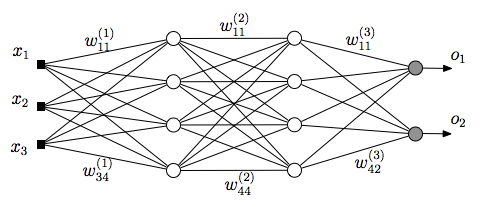
\includegraphics[scale=0.5]{img/MLP}
%     \caption{Paveikslėlio pavyzdys}
%     \label{img:example}
% \end{figure}

% \ref{img:example} Paveikslėlio pavyzdys nurodant jį skaičiumi.

% \subsubsubsection{Straipsnis}
% \subsubsection{Skirsnis}

% Kodo pavyzdys:

\section{Skyrius}
\subsection{Poskyris}
\subsection{Poskyris}

\sectionnonum{Rezultatai ir išvados}
Rezultatų ir išvadų dalyje išdėstomi pagrindiniai darbo rezultatai (kažkas
išanalizuota, kažkas sukurta, kažkas įdiegta), pateikiamos išvados (daromi
nagrinėtų problemų sprendimo metodų palyginimai, siūlomos rekomendacijos,
akcentuojamos naujovės).Kaip pavyzdį galima paanalizuoti pelės judėjimo sekimą naudojant Elm kalbą

\printbibliography[heading=bibintoc]  % Šaltinių sąraše nurodoma panaudota
% literatūra, kitokie šaltiniai. Abėcėlės tvarka išdėstomi darbe panaudotų
% (cituotų, perfrazuotų ar bent paminėtų) mokslo leidinių, kitokių publikacijų
% bibliografiniai aprašai. Šaltinių sąrašas spausdinamas iš naujo puslapio.
% Aprašai pateikiami netransliteruoti.

% \sectionnonum{Sąvokų apibrėžimai}
\sectionnonum{Santrumpos}
Sąvokų apibrėžimai ir santrumpų sąrašas sudaromas tada, kai darbo tekste
vartojami specialūs paaiškinimo reikalaujantys terminai ir rečiau sutinkamos
santrumpos.

\appendix  % Priedai
% Prieduose gali būti pateikiama pagalbinė, ypač darbo autoriaus savarankiškai
% parengta, medžiaga. Savarankiški priedai gali būti pateikiami ir
% kompaktiniame diske. Priedai taip pat numeruojami ir vadinami. Darbo tekstas
% su priedais susiejamas nuorodomis.

\section{Niauroninio tinklo struktūra}
\begin{figure}[H]
    \centering
    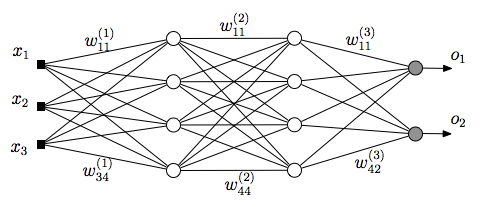
\includegraphics[scale=0.5]{img/MLP}
    \caption{Paveikslėlio pavyzdys}
    \label{img:mlp}
\end{figure}


\section{Eksperimentinio palyginimo rezultatai}
% tablesgenerator.com - converts calculators (e.g. excel) tables to LaTeX
\begin{table}[H]\footnotesize
  \centering
  \caption{Lentelės pavyzdys}
  {\begin{tabular}{|l|c|c|} \hline
    Algoritmas & $\bar{x}$ & $\sigma^{2}$ \\
    \hline
    Algoritmas A  & 1.6335    & 0.5584       \\
    Algoritmas B  & 1.7395    & 0.5647       \\
    \hline
  \end{tabular}}
  \label{tab:table example}
\end{table}

\end{document}
